\section{PEMBAHASAN}
\begin{table}[H]
	\centering
	\caption{Nilai \textit{constant ratio} untuk berbagai kombinasi pasangan}
	\label{tab:cr}
	\begin{tabular}{l l c}
		\toprule
		\textbf{Id} & \textbf{Pasangan} & \textbf{Rata-Rata CR*} \\
		\midrule
		\textit{R1} & a -- c1 & 0,0193233 \\
		\textit{R2} & b -- c1 & 0,0132334 \\
		\textit{R3} & c -- c1 & 0,0132334 \\
		\textit{R4} & a -- c2 & 0,2343343 \\
		\textit{R5} & b -- c2 & 0,3423423 \\
		\textit{R6} & c -- c2 & 0,3423415 \\
		\textit{R7} & a -- c3 & 0,0023444 \\
		\textit{R8} & b -- c3 & 0,0200343 \\
		\textit{R9} & c -- c3 & 0,0234443 \\
		\bottomrule
	\end{tabular}
\end{table}
\lipsum
\begin{figure}[H]
	\centering
	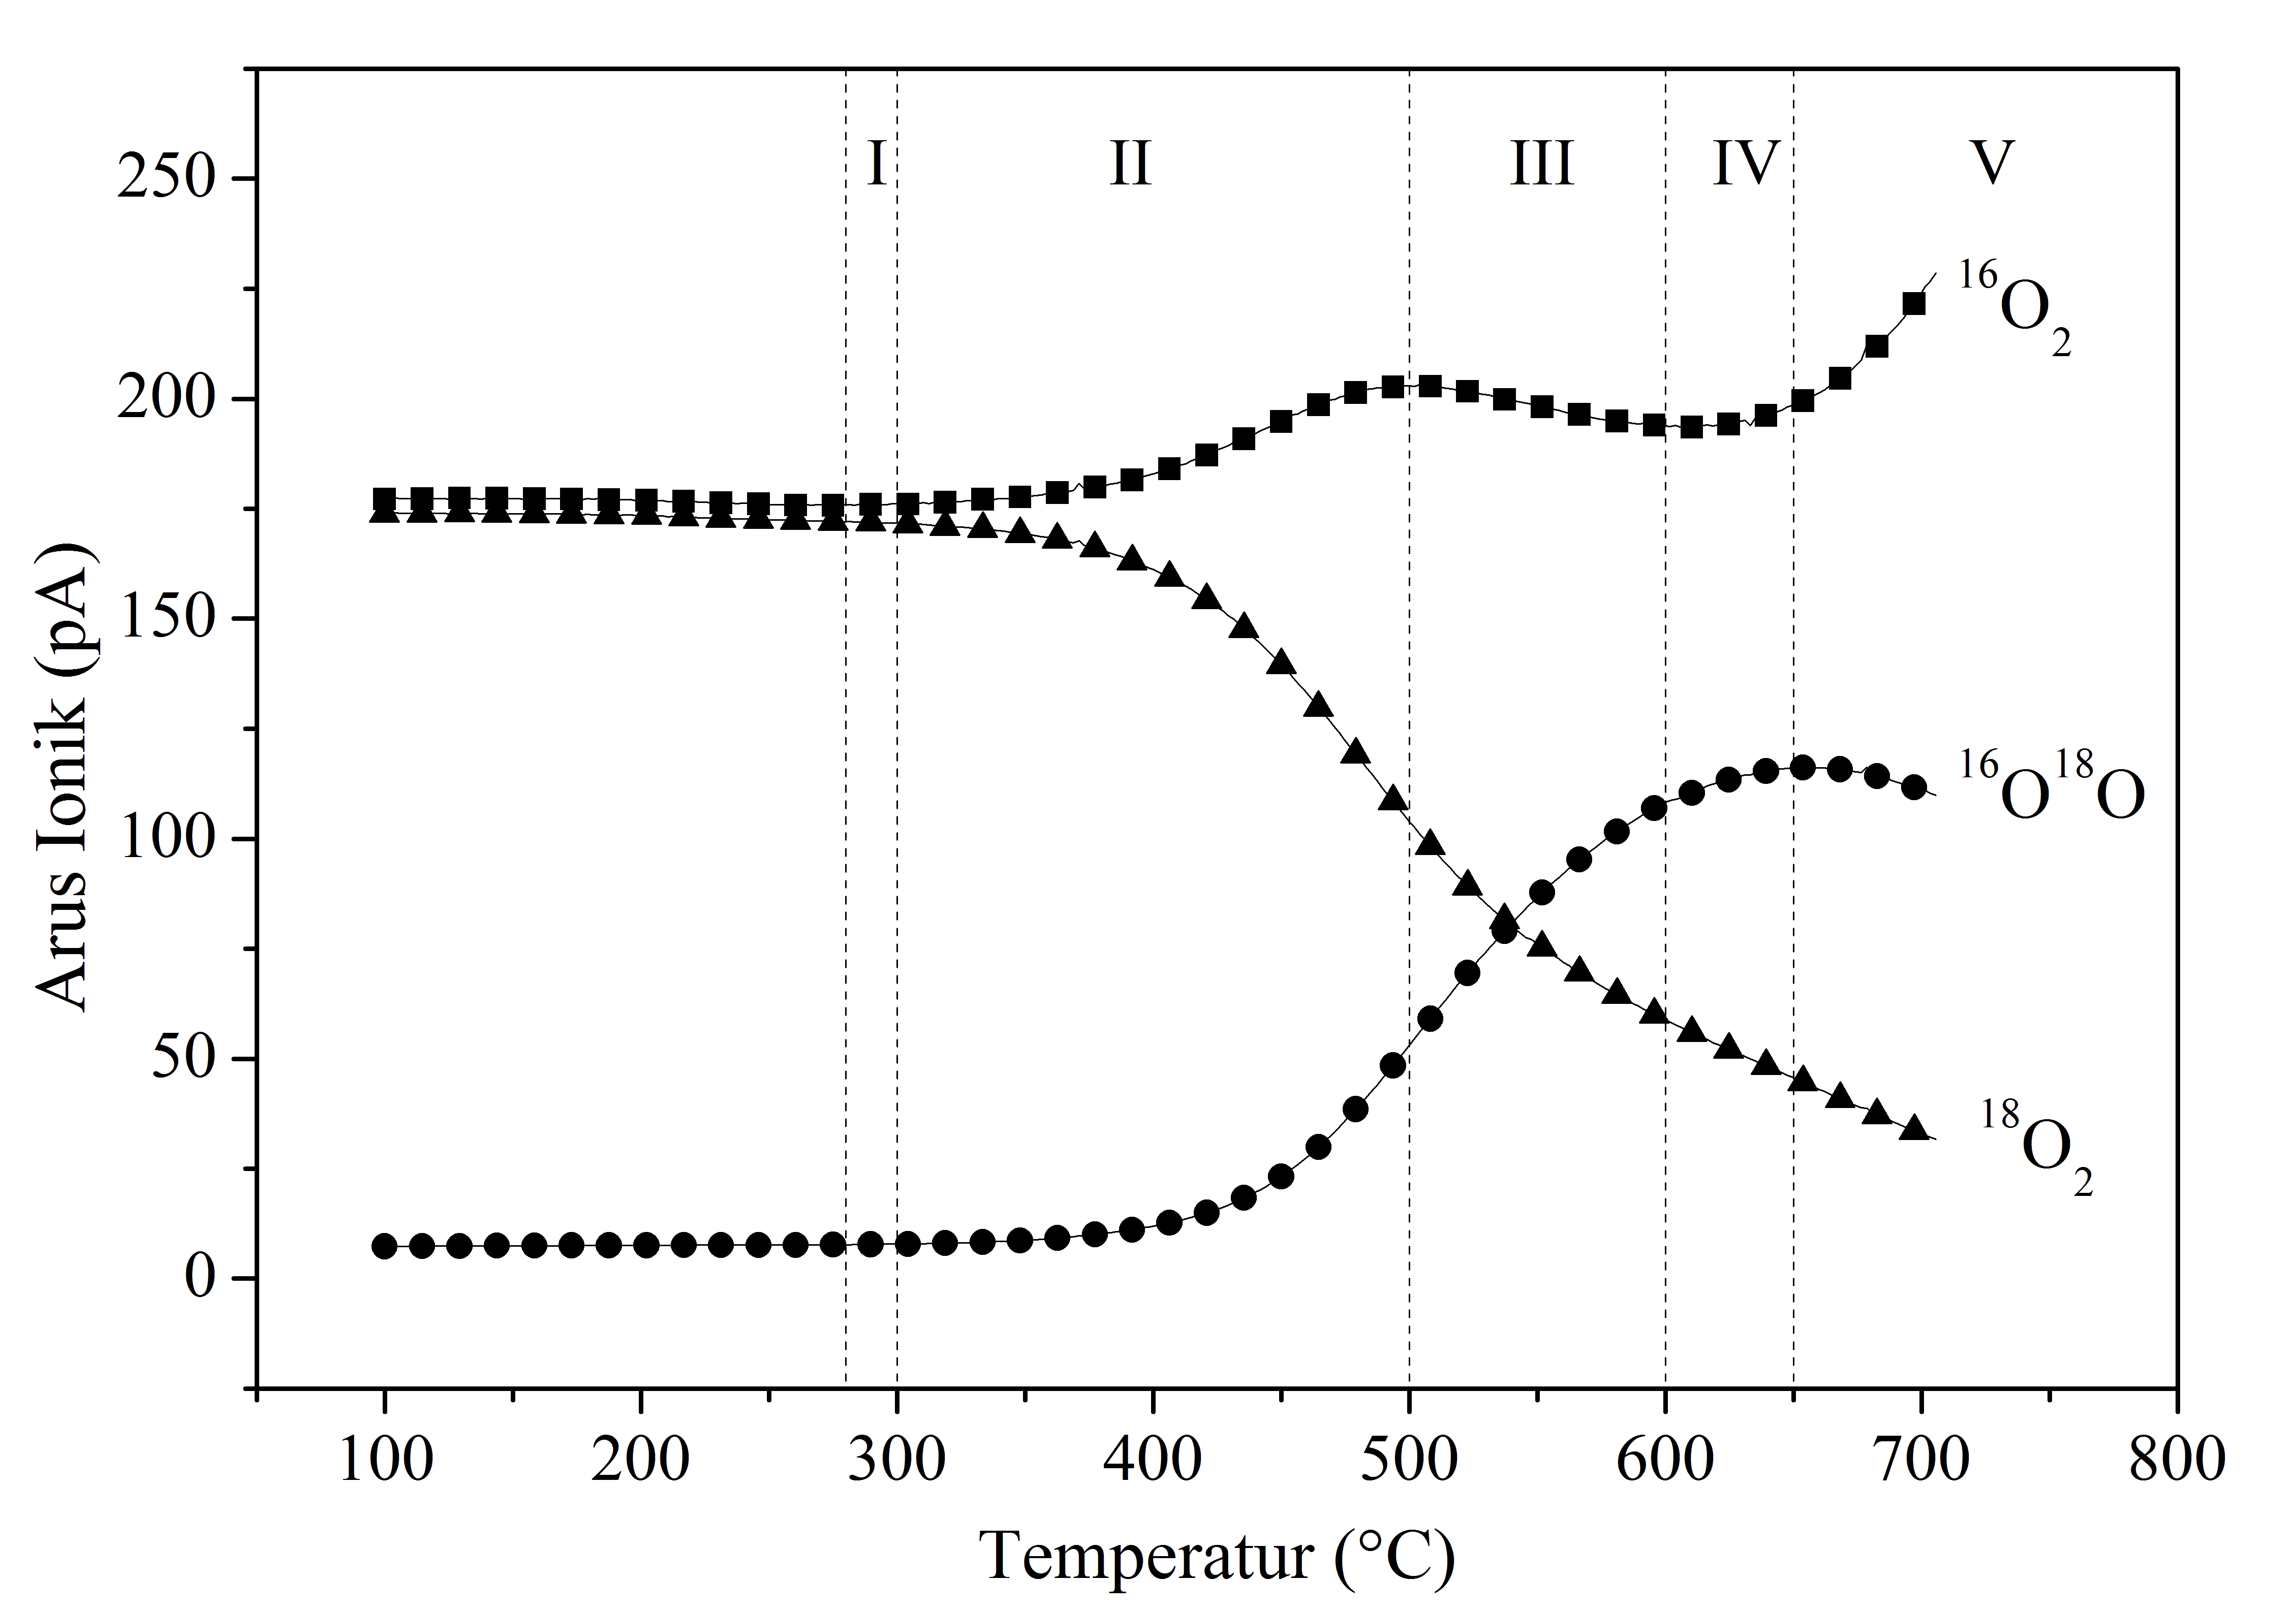
\includegraphics[width=0.7\linewidth]{fig1.png}
	\caption{Example of a inserted image}
	\label{fig:example}
\end{figure}